% !TEX encoding = UTF-8
% !TEX spellcheck = en_US
\documentclass[final]{beamer}
\usepackage[utf8x]{inputenc}
\usepackage{lmodern}
\usepackage{exscale} % fixes some issues with lmodern in math mode
\usepackage[T1]{fontenc}
\usetheme{RJHlandscape}
\usepackage[orientation=landscape,size=a0,scale=1.4]{beamerposter}
\usepackage{tikz}
\usetikzlibrary{shapes,arrows,decorations.markings,positioning}
\tikzset{>=stealth}

\usepackage[absolute,overlay]{textpos}
\usepackage[numbers,compress]{natbib}
\usepackage{booktabs}
\usepackage{multirow}
\usepackage{array}
%\usepackage{wrapfig}
\usepackage{rotating}

\graphicspath{{figures/}}

\newcolumntype{C}[1]{>{\centering\arraybackslash} m{#1} }
\setlength{\TPHorizModule}{1cm}
\setlength{\TPVertModule}{1cm}
\newcommand{\subblock}[1]{\bigskip\textbf{#1}}

\title{Confound and control in language experiments}
\author{Phillip M. Alday  \and Jona Sassenhagen}
\institute{University of South Australia}
\footer{}
%\footer{Live code at \url{https://github.com/jona-sassenhagen/phijona---gamma}}
\date{}

\newcommand{\tikzmark}[3][]{\tikz[overlay,remember picture,baseline] \node [anchor=base,#1](#2) {#3};}
%\DeclareMathOperator*{\Pr}{Pr}
% color blind safe colours, see http://www.cookbook-r.com/Graphs/Colors_%28ggplot2%29/#a-colorblind-friendly-palette
\definecolor{lightorange}{HTML}{E69F00}
\definecolor{lightblue}{HTML}{56B4E9}
\definecolor{lightgreen}{HTML}{009E73}
\definecolor{lightyellow}{HTML}{F0E442}
\definecolor{darkblue}{HTML}{0072B2}
\definecolor{darkorange}{HTML}{D55E00}
\definecolor{darkpink}{HTML}{CC79A7}

\begin{document}
\begin{frame}{} 	


\begin{textblock}{48}(1,7)

\begin{block}{Introduction}
%Experimental research on the neurobiology of language depends on stimulus or participant selection where not all characteristics can be fully controlled, even when attempting strict matching.
Inferential statistics are often used to demonstrate that  confounding covariates do not differ systematically between groups:

\begin{quote}
Animate and inanimate words chosen as stimulus materials did not differ in word frequency (p > 0.05).

Controls and aphasics did not differ in age (p > 0.05).
\end{quote}

%In linguistic stimuli, factors such as word frequency are often correlated with primary factors of interest, such as animacy, or other co-confounds such as word length.
%In clinical studies, factors such as intelligence or socioeconomic status are often correlated with pathology.

%For example, if word length is not significantly different for two conditions, they are considered as matched for word length.
Such a test has high error rates and is conceptually misguided yet is commonly used (67\% of papers attempting to address confounding in a survey of recent Brain and Language issues).
\end{block}

\begin{block}{The stages of failure}
\begin{description}
\item[Philosophy] You can’t accept the null in NHST, only fail to reject it.
\item[Statistics] You’re violating testing assumptions because by design you did not randomly sample and even if had, you're performing inferences on a population you don’t care about.
\item[Pragmatics] You’re failing to perform the inference you actually care about (the impact of the confounding covariate on the dependent measure).
\end{description}
\end{block}

\begin{block}{Do you see what you've been missing?}
\begin{center}
\begin{tabular}{l l l }
\centering
What you're testing & What you worry about & What you care about \\
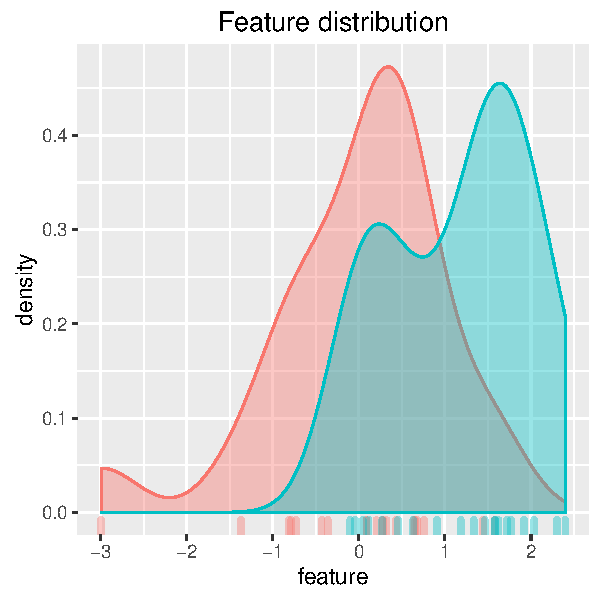
\includegraphics[width=0.3\textwidth]{feature.pdf}  & 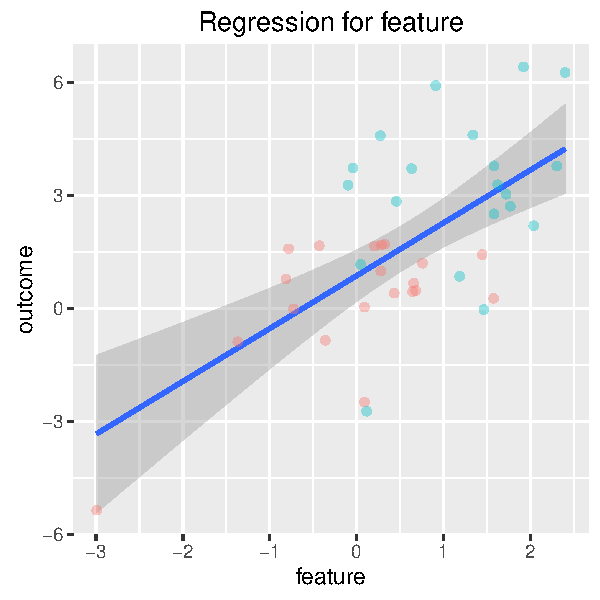
\includegraphics[width=0.3\textwidth]{feature_regression.pdf} & 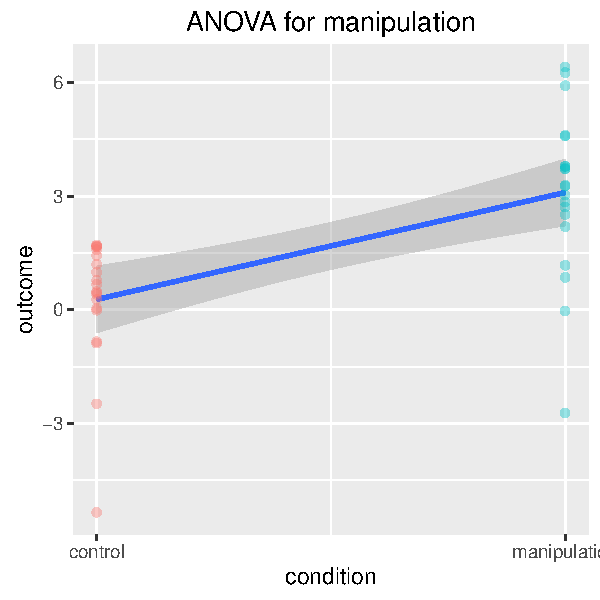
\includegraphics[width=0.3\textwidth]{anova.pdf} \\
\end{tabular}

What you should be doing:\\
 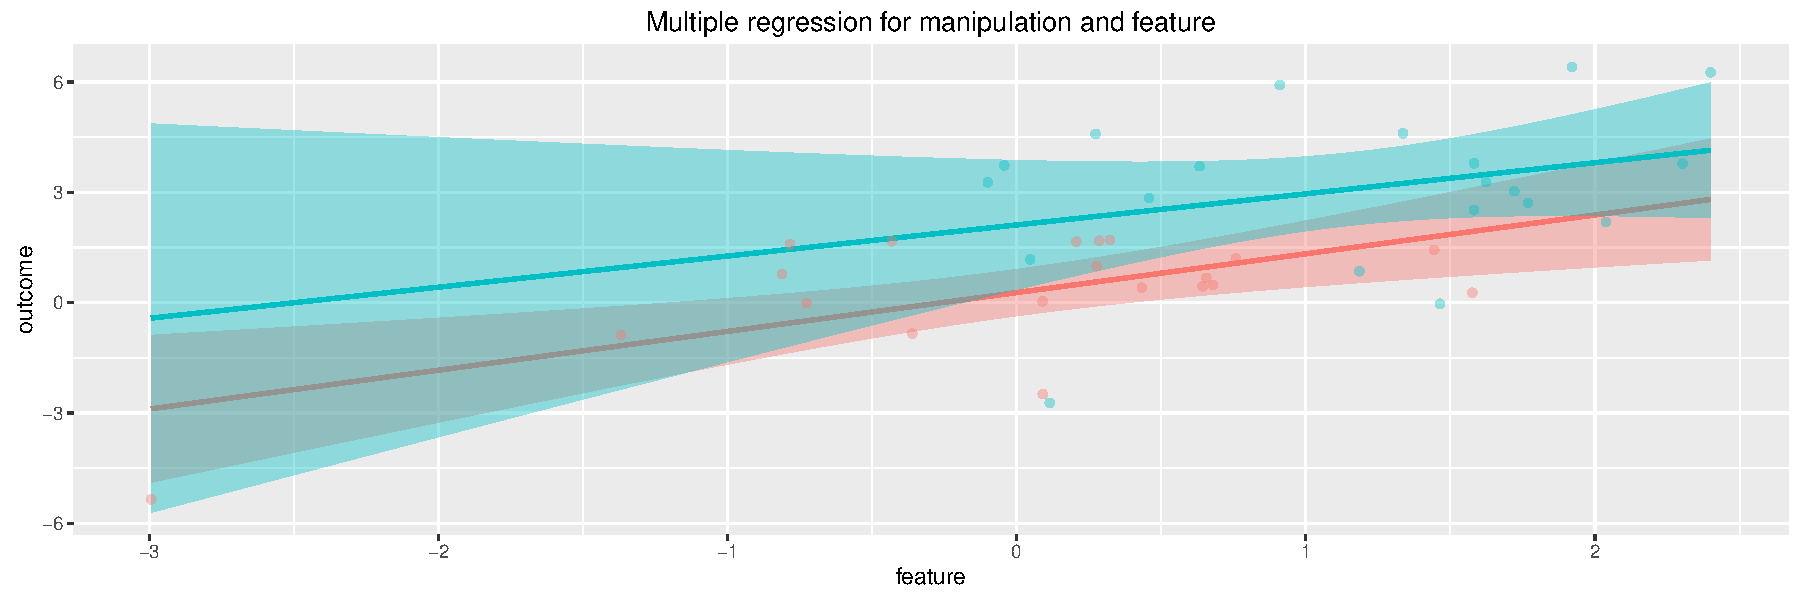
\includegraphics[width=1\textwidth]{multiple_regression.pdf} 
\end{center}

\tiny
\hfill Effect size: Cohen's $d=2$, confound size Cohen's  $d=1$, confound-outcome correlation: Pearson's $r=1$

\end{block}

\begin{block}{Interesting Interactions}
Complex interactions make completely unconfounded studies difficult. 
For example, marked constructions are generally less frequent than unmarked ones, leading to the claim that observed differences in processing are frequency effects.
Modelling our confounds directly allows us to examine the piecewise contributions from the experimental manipulation and the 'confound'.

\vspace{.38cm}
\end{block}

\end{textblock}

\begin{textblock}{48}(50.5,7)

\begin{block}{Wasted stimuli}
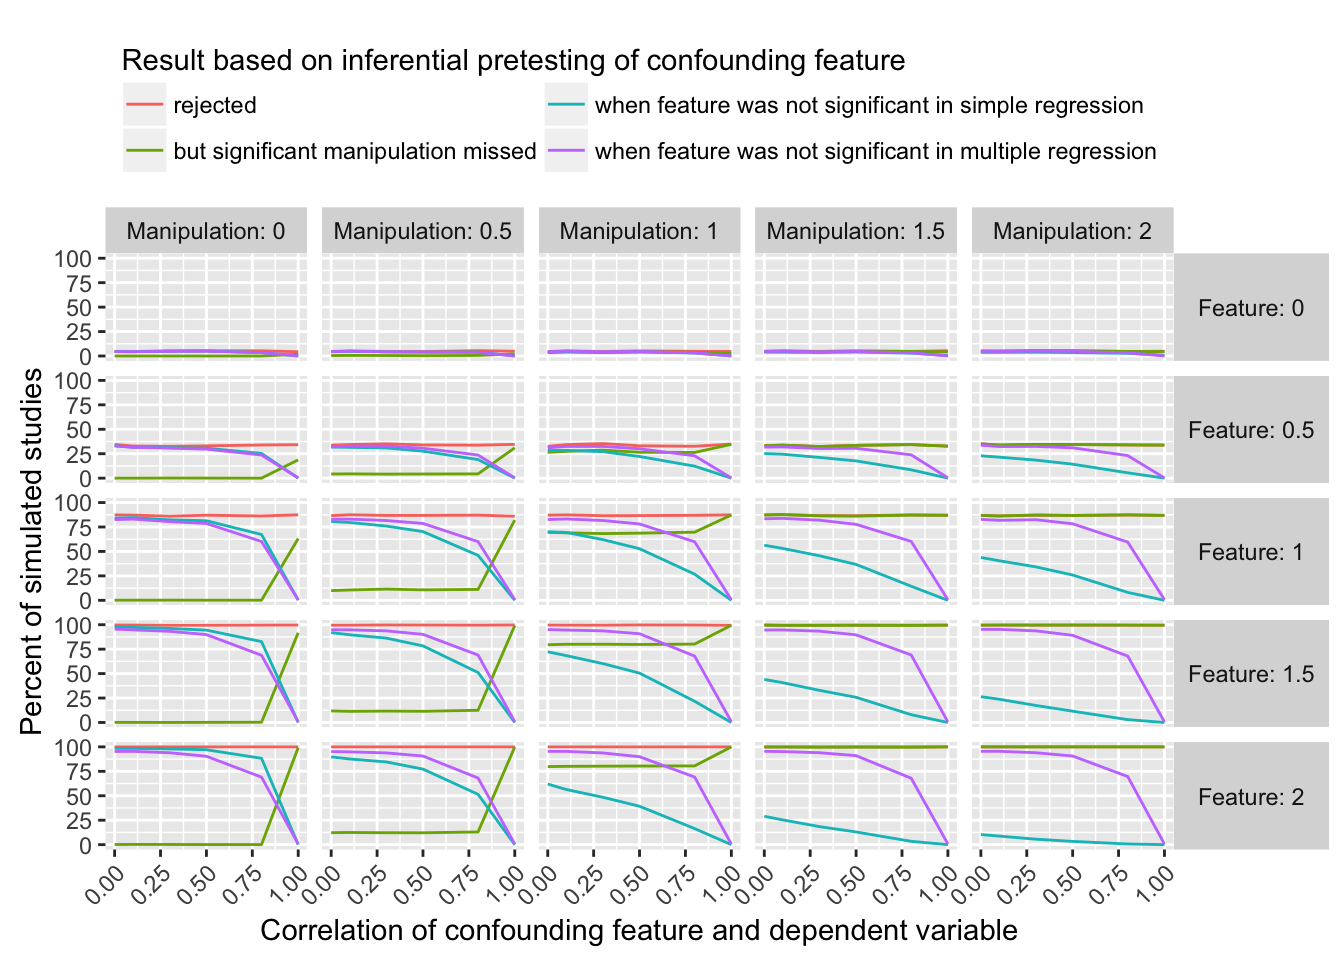
\includegraphics{rejections.png}
\end{block}

\begin{block}{Missed confounds}
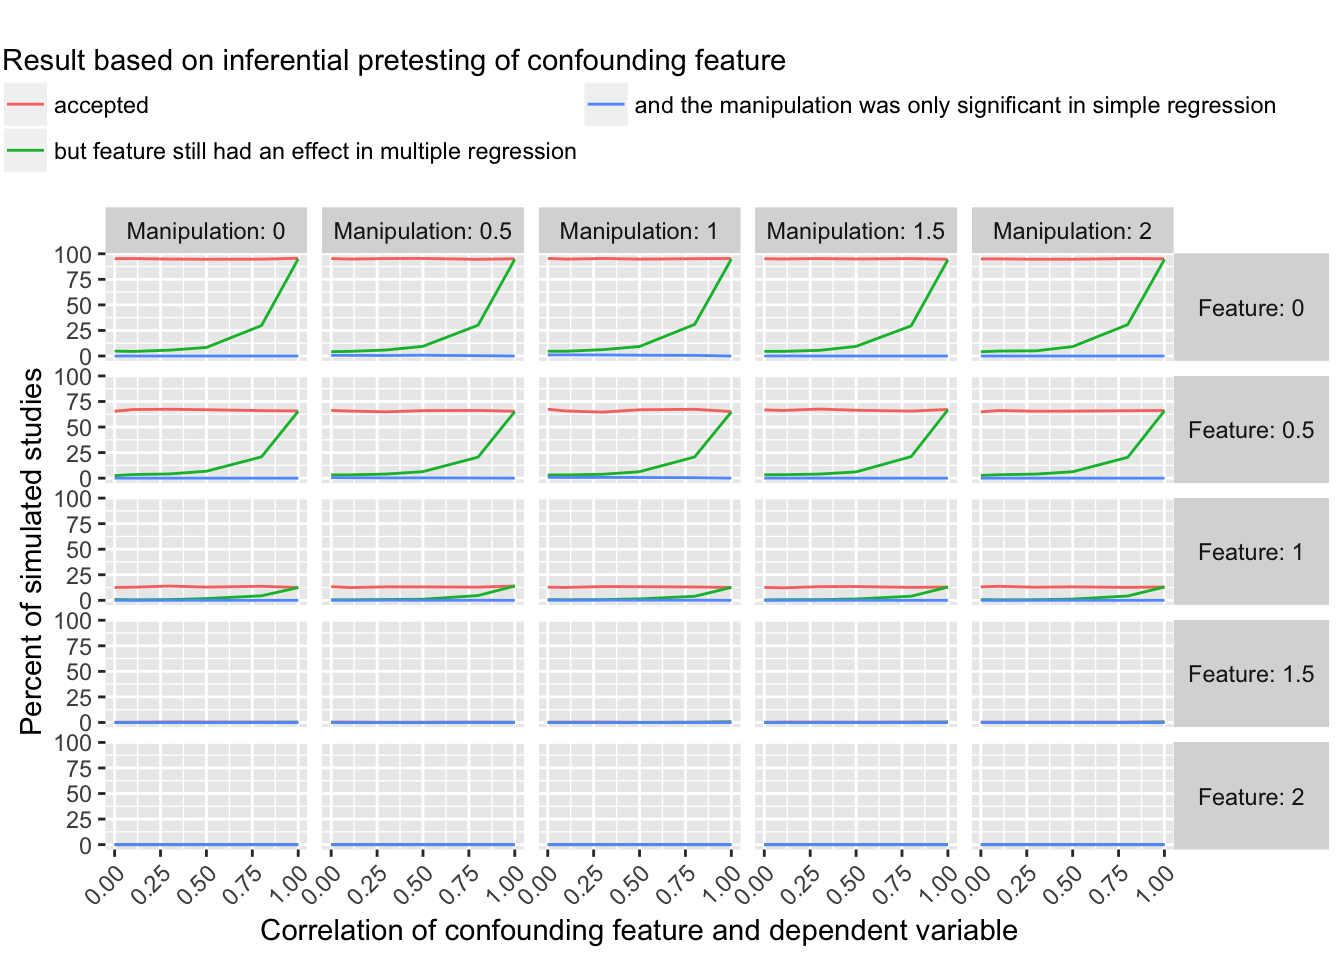
\includegraphics{acceptances.png}
\end{block}

\end{textblock}

\begin{textblock}{18}(100,7)

\begin{block}{Getting things under control}
Match descriptive statistics (measures of central location such as mean and median, as well as variance).

\vspace{0.8cm}

Include a 'nuisance' covariate in an appropriate statistical model, such as a mixed-effects model.

\vspace{0.8cm}

The actual impact of the confound can be examined both by its associated model parameters and by comparison between models with and without the nuisance covariate.

\vspace{0.8cm}

\textbf{Appropriate model selection is the way to determine the influence of confounds.}

\end{block}

%\begin{block}{Literature}
%\tiny
%\bibliographystyle{poster}
%\bibliography{snl2016.bib}
%\vspace{0.25cm}
%\end{block}

\begin{block}{Try the app!}
\centering

\includegraphics[width=0.55\textwidth]{shinyapps-url.eps}
%
%http://rpubs.com/palday/statfail
\end{block}

\begin{block}{Read the preprint!}
\centering

\includegraphics[width=0.55\textwidth]{arxiv-url.eps}
%

\end{block}

\begin{block}{}
\begin{tabular}{c c }

\includegraphics[width=.55\linewidth]{logo_unisa_RGB-blue.png} &   
\includegraphics[width=.3\linewidth]{cnl-color.eps}  \\

\includegraphics[width=.4\linewidth]{logo_frankfurt_square.png} & 
\includegraphics[width=.4\linewidth]{logo_fiebach_lab.png} \\
\end{tabular}

\vspace{0.4cm}

%\includegraphics[width=.9\linewidth]{logo_mainz_new.eps}
\end{block}


\end{textblock}

\end{frame}
\end{document}
